% include the figures path relative to the master file
\graphicspath{{./content/experiments/figures/}}

\section{Experiments and Results}
This section presents our setup, the designed experiments, the obtained
results, the difficulties faced during the experiments and our provided
solutions.

\subsection{Setup}
\label{sec:setup}
The setup used in our experiment is based on fig.~\ref{fig:rotation}.
%However instead of \gls{uav}, a camera tripod was used.
For the presented experiments, we considered that $R_{vi}$ between \gls{imu} and
\gls{uav}, as well as initial pose of the \gls{uav} in the world frame were
identity.  To be able to using the \gls{imu} recordings as \gls{gt}, this device was
calibrated with the camera using kalibr toolbox~\cite{furgale2013unified,
  furgale2012continuous}. The polarimetric camera with fisheye lens was also
calibrated according to~\cite{kannala2006generic}.

Using the explained setup two dataset of synthetic and real images were
created. The results obtained using these two dataset are presented in
Exp.~\ref{exp1} and Exp.~\ref{exp2}, respectively.

\subsection{Experiment~1}
\label{exp1}
This experiment is based on synthetic data. Indicating that \gls{aop} and
\gls{dopl} images for sky regions were synthetically created using the \gls{imu}
recordings obtained during real acquisition. Figure~\ref{fig:aop-dop-syn} shows
an example of this dataset.

\begin{figure}
    \centering
    \subfigure[\gls{aop}]{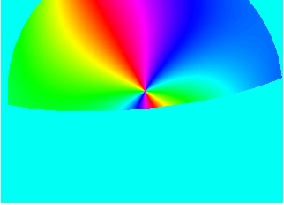
\includegraphics[width= 0.22\textwidth]{./content/experiments/figures/aop-no-noise.png}}\hfill
    \label{fig:aop-syn}
    \subfigure[\gls{dopl}]{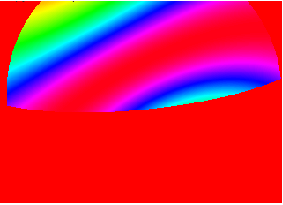
\includegraphics[width=0.22\textwidth]{./content/experiments/figures/dop-no-noise.png}}
    \label{fig:dop-syn}
    \hspace*{\fill}
    \caption{Synthetically created \gls{aop} and \gls{dopl} images of sky
      region for yaw, pitch and roll angle of 1.8, -0.2 and 0.1, respectively.}
    \label{fig:aop-dop-syn}
\end{figure}


\subsection{Experiment~2}
\label{exp2}







%%%Local Variables:
%%% mode: latex
%%% TeX-master: t
%%% End:
